\section{Human experimental details}
\label{sec: experiment}


\subsection{Participants} \label{sec: A.1}
Twenty-seven participants (15 females; age range: 18–25 years) were recruited for the experiment. Three participants voluntarily withdrew due to persistent difficulties with the learning task and were excluded from all subsequent analyses. All participants had normal or corrected-to-normal vision, reported no color vision deficiencies, and had no known history of psychiatric disorders. Written informed consent was obtained prior to participation, and monetary compensation was provided following the completion of the study.

\subsection{Stimuli} \label{sec: A.2}
To enable the generation of a virtually infinite set of stimuli within a four-dimensional continuous feature space, we developed a custom 2D line-drawing stimulus generation program, inspired by prior work~\cite{OLMAN2004227, NIPS2007_89d4402d}. Crucially, all stimuli were entirely novel, minimizing reliance on prior knowledge and providing a clean slate for learning. Each stimulus is composed of five parts: a fixed-length body (3.8° visual angle) and four parametrically varying features—head, neck, tail, and legs—whose lengths vary continuously from 0.25 to 1.25 times the body length. Each stimulus is rendered in either a left- or right-facing orientation. To eliminate any cues to 3D structure, all line angles were fixed, ensuring that morphological variation arises solely from differences in feature lengths.


\subsection{Procedure and design} \label{sec: A.3}
The experiment was conducted on a 27-inch LCD monitor with a resolution of 1920×1080 pixels and a refresh rate of 100 Hz. All stimuli were presented against a uniform gray background (RGB: 127, 127, 127). Experimental procedures were implemented using MATLAB (MathWorks Inc., Natick, MA, USA) in combination with Psychtoolbox-3. Participants used a headrest during tasks to minimize head movements and maintain a 60 cm viewing distance, ensuring a 3.8° visual angle for the stimulus body length. Behavioral responses were recorded via keyboard input, while verbal reports were collected using a professional-grade audio recorder. 

\subsubsection{Preparation task}
Prior to the main learning task, participants completed two preparatory tasks: a \textbf{free exploration task} (Fig. \ref{fig:S1}A), followed by a \textbf{perceptual calibration task} (Fig. \ref{fig:S1}B). 

The \textbf{free exploration task} was designed to familiarize participants with the length range of each feature dimension. In the task, participants manipulated an interactive stimulus by dragging morphological nodes (head, neck, tail, or legs) while the body remained fixed as a reference. Leg adjustments automatically synchronized the remaining three limbs to preserve quadrupedal symmetry. A flip button enabled left-right orientation changes. Task duration was limited to 5 minutes.

We employed a \textbf{perceptual calibration task} to estimate \textit{just-noticeable differences} (JNDs) along each feature dimension for individual participants. This involved a pairwise stimulus matching paradigm. On each trial, participants viewed two stimuli--a \textit{reference} stimulus and an \textit{adjustable} stimulus--displayed in either the same (e.g., left-left) or opposite orientations (e.g., left-right) to eliminate orientation-specific estimation bias. Each stimulus was created by randomly combining four features, with each feature dimension uniformly sampled at seven levels across its full range. Stimuli were vertically jittered on screen to prevent pixel-wise template matching. Using the same interactive interface as the free exploration task, participants adjusted the modifiable stimulus via mouse-drag to match the reference stimulus as closely as possible, regardless of vertical position or horizontal orientation. This design ensured responses reflected perceived feature differences rather than superficial pattern matching.

During the perceptual calibration, participants completed 192 trials covering all pairwise comparisons across the seven sampling levels for each feature. Mandatory rest periods (minimum 1 minute) were enforced after every 24 trials to prevent fatigue. For each feature, JND were estimated by calculating the distribution of discrepancies between \textit{final-adjusted} and \textit{reference} stimuli across all trials. The resulting means and standard deviations of these perceptual errors per feature parameterized individualized perceptual noise in subsequent computational modeling.

\begin{figure}[t]
    \centering
    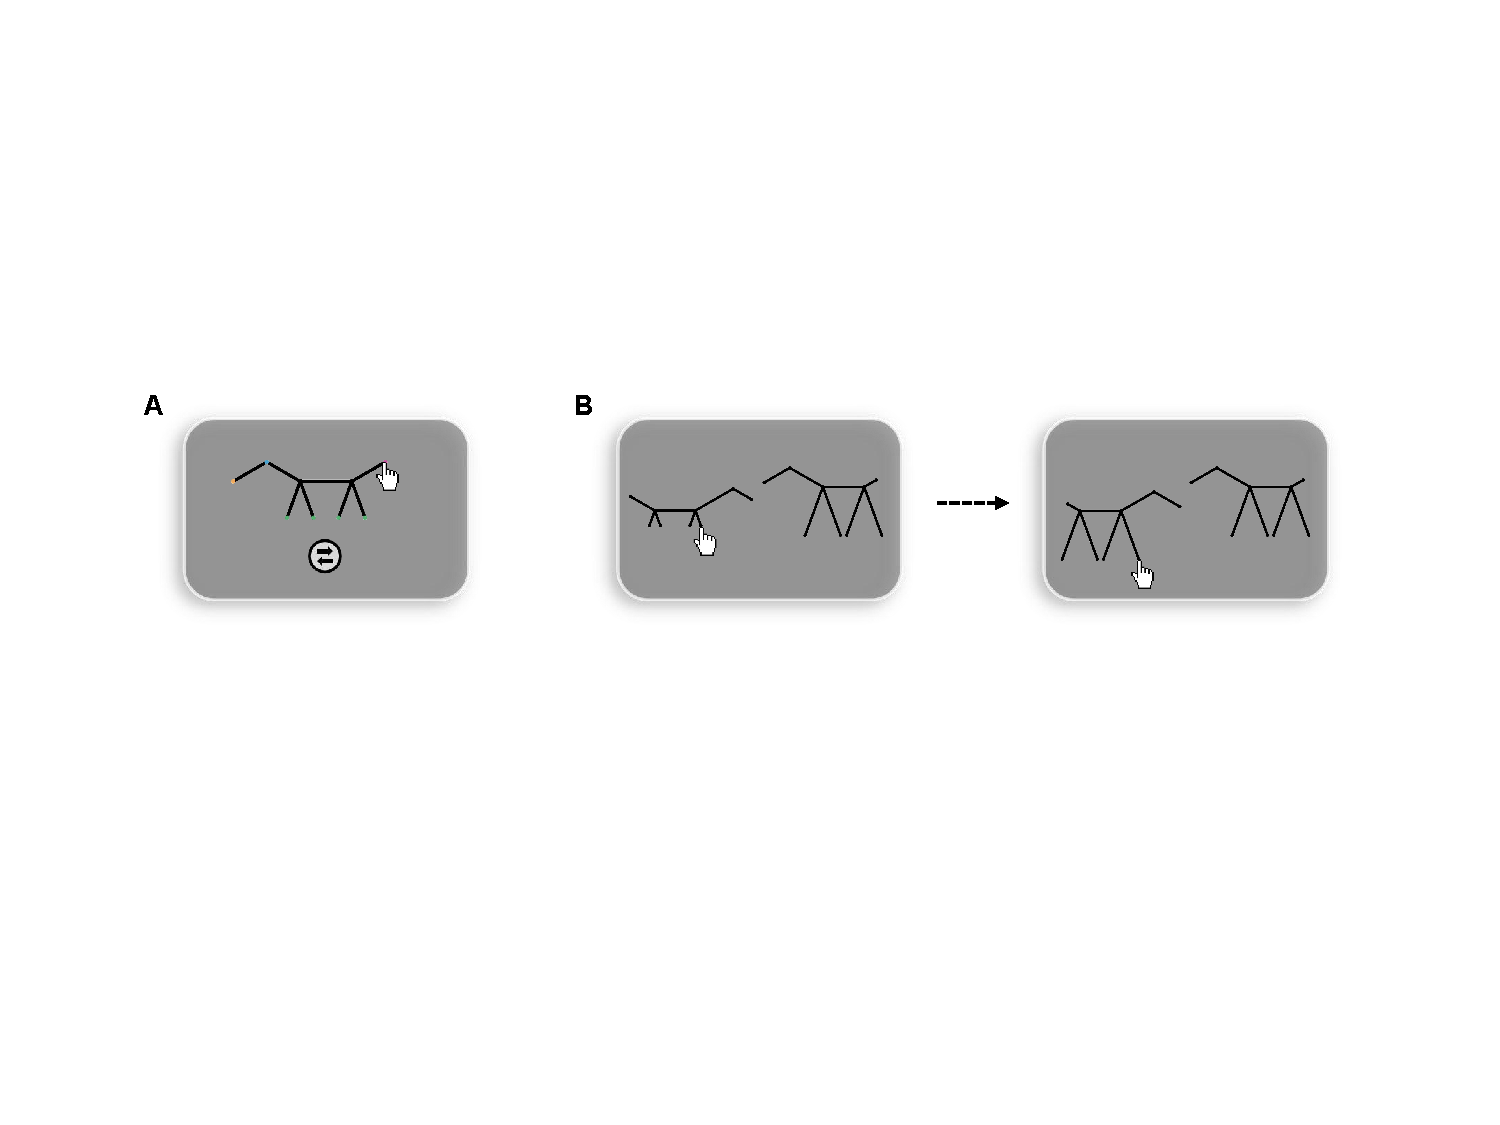
\includegraphics[width=1\textwidth, trim=2cm 8.3cm 2cm 6.6cm, clip]{figs/FigureS1.pdf}
    \caption{Preparation tasks. \textbf{(A)} Free exploration task: participants use the mouse to drag nodes or click the flip button to toggle the left–right orientation of each stimulus. \textbf{(B)} Perceptual calibration task: participants adjust the left stimulus to match the right stimulus as closely as possible in shape.}
    \label{fig:S1}
\end{figure}

\subsubsection{Learning task}
Participants were trained to categorize stimuli with infinite variations in dimensional feature space into a limited number of distinct groups. This design mirrors real-world challenges where learners must solve an ill-posed inverse problem: iteratively selecting and re-weighting relevant features from rich sensory inputs to derive low-dimensional categorical labels. 

Three different learning conditions were implemented using a between-subjects design. In \textbf{Task 1}, a simple two-category rule was based on a single randomly assigned feature, with the midpoint of the full range serving as the deterministic boundary between categories F and J (e.g., F = leg length > 0.5, J = leg length < 0.5, in a normalized range from 0 to 1). \textbf{Task 2} employed a four-category rule requiring integration of three features to form a hierarchical structure: four subordinate categories (F, G, H, J) nested under two basic-level categories (e.g., F\&H vs. J\&G), again using midpoint boundaries. For example, leg length (long vs. short) determined the basic-level categories, while combinations of neck and head lengths determined the four subordinate categories within each basic level. Feedback signals explicitly revealed the nested structure: 1 = correct at both levels, 0.5 = correct at basic level only, 0 = incorrect at both levels. \textbf{Task 3} used the same four-category structure but without hierarchical feedback—participants received binary feedback (1 = correct, 0 = incorrect) based solely on subordinate-level accuracy. Most of the participants in this condition reported not recognizing the hierarchy after successful learning. Crucially, participants received no information on what features or rules to use for categorization prior to training.

An adaptive learning procedure was implemented to avoid excessively long training sessions. Training blocks consisted of 64 trials each. We computed learning accuracy and \textit{d-prime} \footnote{The \textit{d-prime} ($d'$) score for each category was computed as $d' = Z(\text{hit rate}) - Z(\text{false alarm rate})$, where $Z(\cdot)$ denotes the inverse cumulative distribution function of the standard normal distribution.} for each category per block, excluding trials with ambiguous stimuli (any feature value within the 0.45–0.55 range). Based on calculated \textit{d-prime} values, stimulus distributions were adaptively adjusted for subsequent blocks: better-learned categories (higher \textit{d-prime}) appeared less frequently. This resulted in individualized, adaptive stimulus sequences for each participant. Training continued until participants achieved >90\% accuracy for all categories within a block or reached the 25-block limit. All participants except voluntary withdrawals successfully completed the task within these limits. To prevent fatigue, mandatory rest periods (minimum 1 minute) were enforced every 16 trials within each block. See Fig. \ref{fig:S2} for each individual's learning performance in Task 2 and Task 3, reflecting the similar variability in Task 1 as we reported in Fig. 1D.

\begin{figure}[htp!]
    \centering
    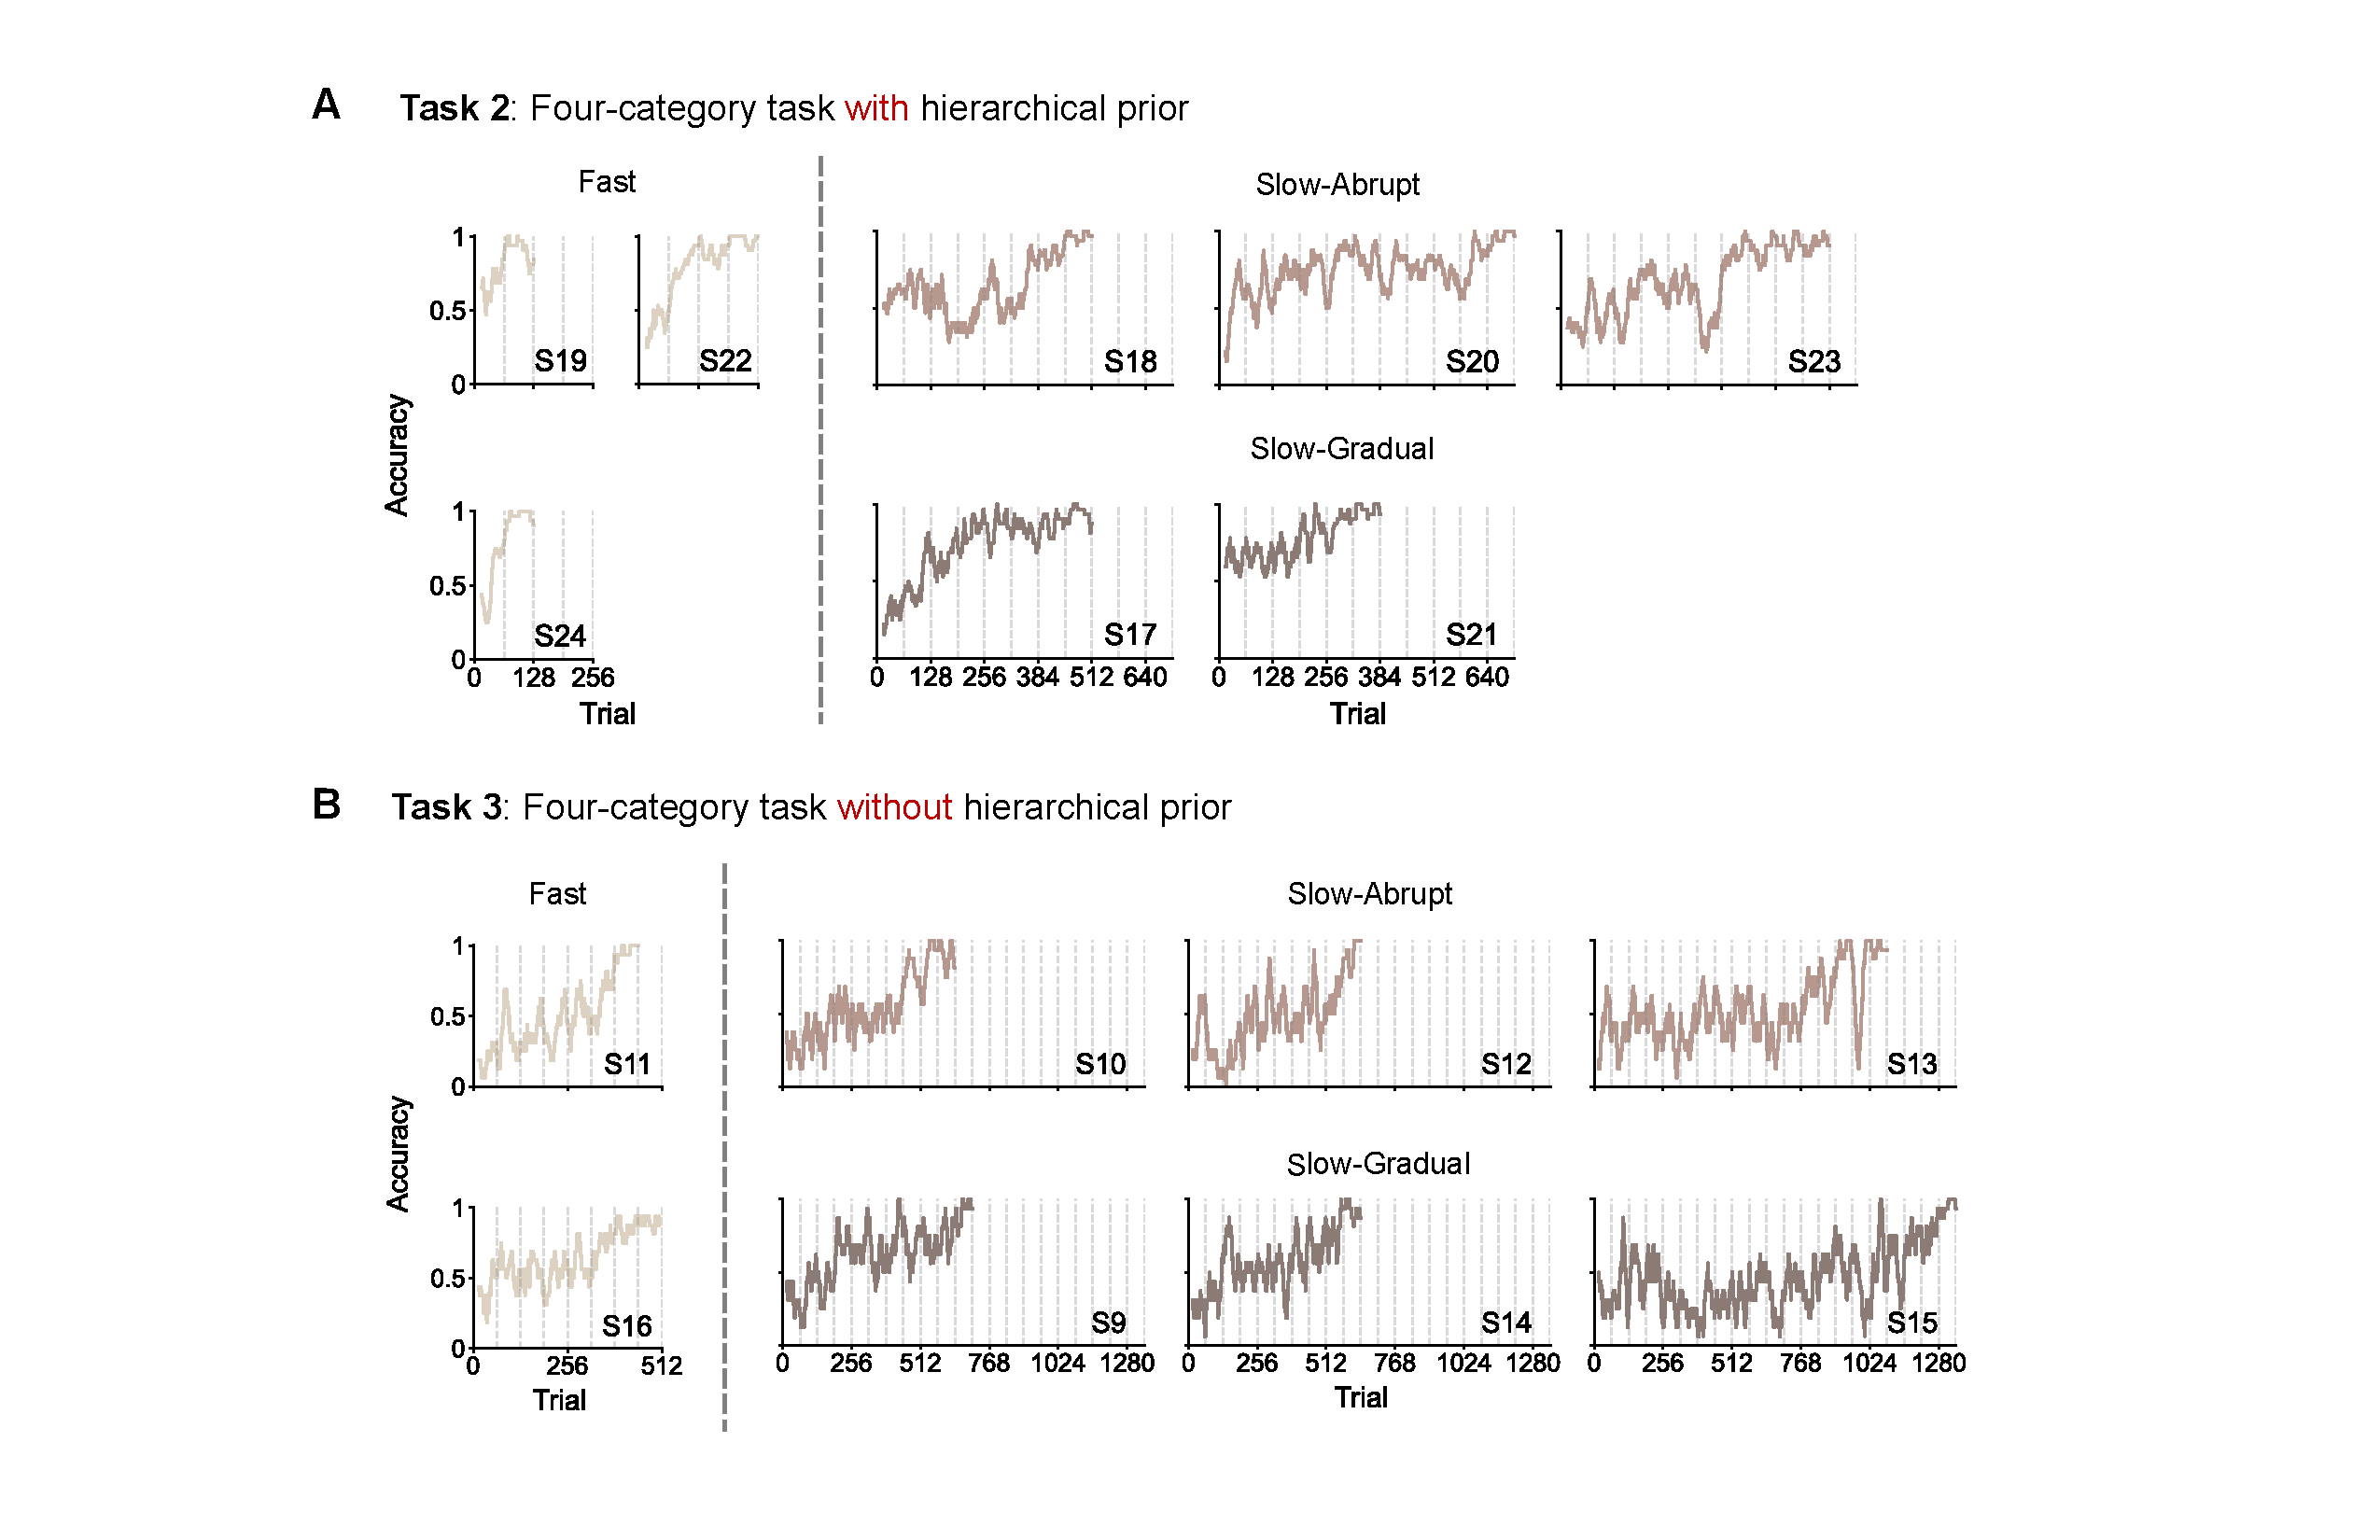
\includegraphics[width=1\textwidth, trim=5cm 1.5cm 5cm 1.5cm, clip]{figs/FigureS2.pdf}
    \caption{Learning performance in \textbf{(A)}Task 2  and \textbf{(B)}Task 3. Participants in each task could be broadly classified into three groups--fast (lightest brown), slower but abrupt (medium brown), and slower and gradual (darkest brown), as in Task 1.}
    \label{fig:S2}
\end{figure}


\subsection{Oral report coding} \label{sec: A.4}

In each learning trial, participants verbally reported the reasons for their category choice immediately after making a decision and prior to receiving feedback (with invalid or missing reports accounting for only 0.008\% of trials). We extracted structured internal representations from these verbal reports using a rule-based natural language parser that mapped spoken descriptions onto the four-dimensional feature space (see Table~\ref{tab:S1}). By concatenating these trial-wise representations, we reconstructed the learning trajectories shown in Fig. 1E of the main text.

Specifically, each report was first segmented into multiple expressions using commas as delimiters. For each expression, we identified and encoded the following components: (1) the description type (e.g., direct, comparative, superlative, exclusionary), (2) the referenced feature(s) (head, neck, tail, or legs), and (3) the described magnitude (e.g., “long,” “short,” “longer,” “longest”). Each expression was then translated into a numerical vector reflecting the inferred \textit{prototypical} values or weights associated with the mentioned features.  At the trial level, the final value for each feature was computed as the average of all values assigned to it across expressions; features not mentioned in any expression were assigned a default value of 0.5.


\begin{table}[htbp!]
\centering
\caption{Mapping rules from verbal reports to feature-space values}
\begin{tabularx}{\textwidth}{l X p{2.2cm} p{2cm}}
\toprule
\textbf{Description type} & \textbf{Example phrase (translated)} & \makecell[l]{\textbf{Mapped}\\ \textbf{feature(s)}} & \makecell[l]{\textbf{Prototypical}\\ \textbf{value(s)}} \\
\midrule
Direct & \makecell[l]{“The legs are long”\\ “The tail is short”\\ “The head is moderate”} & \makecell[l]{legs\\ tail\\ head} & \makecell[l]{0.75\\ 0.25\\ 0.5} \\
Comparitive & “The neck is longer than the head” & neck, head & \makecell[l]{neck = 2/3,\\ head = 1/3} \\
Overall & “All parts are short” & all features & 0.25 \\
Exclusive & “All parts are short except the tail” & all features & \makecell[l]{tail = 0.75,\\ others = 0.25} \\
Superlative & “The head is the longest” & all features & \makecell[l]{head = 0.8,\\ others = 0.4} \\

\bottomrule
\end{tabularx}
\label{tab:S1}
\end{table}